\subsection{\labeltext[Diagrama de Estados - Devolução]{Diagrama de estados - Devolução}{es:251}}

\begin{figure}[H]
	\centering
	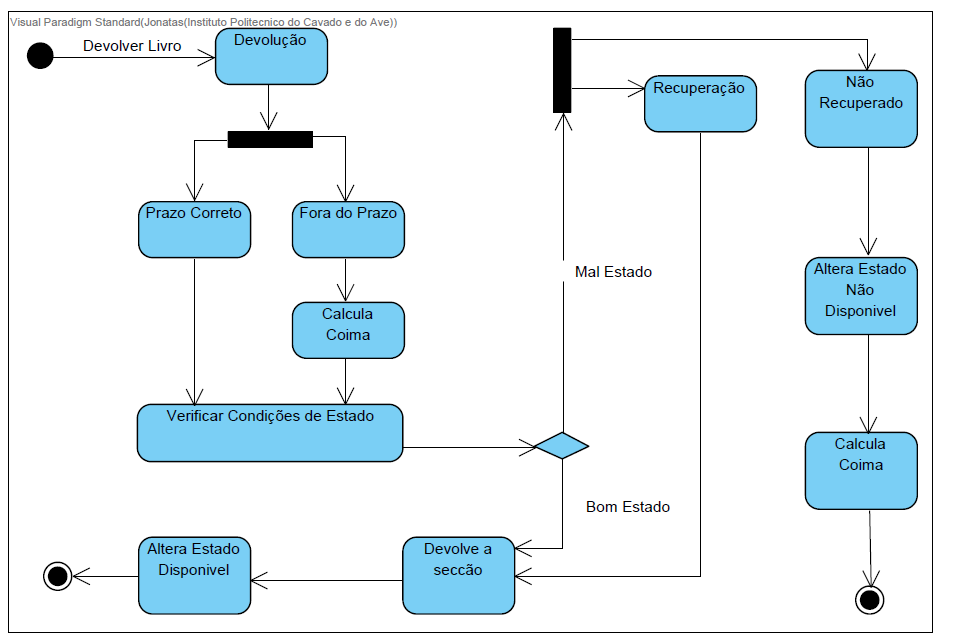
\includegraphics[width=1\linewidth]{./img/Diagrama_E/DE_Devolucao.png}  % largura percentual 
	\caption{\ref{es:251}}
	\label{fig:chap251}
\end{figure}

\par O diagrama de “Devolução” inicia no estado "Devolução", quando este está no “Prazo Correto” o estado segue para “Verificar condições de Estado”, na ocasião de estar “Fora do Prazo” o estado altera para “Calcula Coima”  e, segue para “Verificar condições de Estado”, quando este livro está em boas condições o estado altera para “Devolve a Secção” e após “Altera Estado para Disponível” e finaliza o processo, quando o livro encontra-se em mal condição o estado altera para “Recuperação” e caso seja possível o reparo volta para o estado de “Devolve a Secção”, já no caso de “Não Recuperado” o estado “Altera Estado para Não Disponível” e segue para “Calcula Coima” após o processo finaliza.
